\chapter{The Three-body Problem}
Two-body scattering processes basically concern two different situations, elastic and inelastic collisions. For the three-body problem, solving the three-body Schr{\"o}dinger equation is more involved. The enhanced complexity is mainly due to the increased number of fragmentation channels in the scattering processes. In addition to the triatomic fragmentation channel (1+1+1), there are three possible atom-dimer fragmenation channels (1+2). This makes the construction of permutation symmetric wavefunctions highly non-trivial. 

There are different routes for solving the three-body problem and they involve either solving the three-body Schr{\"o}dinger equation or solving the Faddeev equation, which is equivalent to solving the three-body Schr{\"o}dinger equation in configuration space. Irrespective of the specific method of choice for solving the three-body system, most approaches start with the same steps. This includes separating out the center-of-mass motion and then defining a set of relative coordinates. A convenient choice for the three-body problem is mass normalized Jacobi coordinates, since this removes the mass factors in the kinetic energy operator. 

Atomic units (a.u.) will be used throughout this theisis. There are four fundamental atomic units -- the electron rest mass $m_e$, the elementary charge $e$, the reduced Planck's constant $\hbar$, and the Coulomb force constant $k_e$ -- which numerical values are unity by definition, i.e. $m_e = e = \hbar = k_e = 1$. Derived atomic units include dimensions of length and energy, which are expressed in terms of the Bohr radius $a_0$ and the Hartree $E_h$.    

\section{Mass Normalized Jacobi Coordinates}\label{MNJC}
The spatial position of three particles in $\mathbb{R}^3$ are fixed by nine coordinates $x_{\alpha}^{i}$, where $i(=1,2,3)$ labels the particles, and $\alpha(=1,2,3)$ their Cartesian space coordinates, respectively. Let $\mathbf{x}_i$ and $m_{i}$ be the position vector and mass of the $i$th particle in the laboratory frame. If the total mass $M$, the three particle reduced mass $\mu$, and the normalizing constants $d_{k}$ $(k=1,2,3)$ are defined by

\begin{align}
M &= \sum_{i=1}^{3}m_i,  \label{eq:3,1} \\
\mu^2 &= \prod_{i=1}^{3}m_i/M,  \label{eq:3,2}\\
d_k^2 &= \frac{m_k}{\mu}\frac{(m_i+m_j)}{M},  \label{eq:3,3}
\end{align}
then a set of mass scaled Jacobi coordinates and the center-of-mass coordinate can be defined as

\begin{align}
\mathbf{r}_k &= d^{-1}_k(\mathbf{x}_{j}-\mathbf{x}_{i}),  \label{eq:4,1} \\
\mathbf{R}_k &= d_k\Big[\mathbf{x}_{k}-\frac{(m_{i}\mathbf{x}_{i}+m_{j}\mathbf{x}_{j})}{m_{i}+m_{j}}\Big],  \label{eq:4,2}\\
\mathbf{X}_{cm} &= \frac{1}{M} \sum_{i=1}^{3} m_{i} \mathbf{x}_{i},  \label{eq:4,3}
\end{align}   
in which the indices $i,j,k$ are cyclic permutations of $(1,2,3)$ and where $\mathbf{r}_k$ is the scaled vector from particle $i$ to $j$, and $\mathbf{R}_k$ is the scaled vector from the centre-of-mass of the pair $ij$ to particle $k$, see \cref{fig:1}.
\begin{figure}
	\centering
	 \documentclass{standalone}
 \usepackage{tikz}
 \usepackage{tikz-3dplot}
 \usetikzlibrary{calc}
 
 \begin{document}
 
  %Angle Definitions
%-----------------

%set the plot display orientation
%synatax: \tdplotsetdisplay{\theta_d}{\phi_d}
\tdplotsetmaincoords{60}{110}

%define polar coordinates for some vector
%TODO: look into using 3d spherical coordinate system
\pgfmathsetmacro{\rvec}{.8}
\pgfmathsetmacro{\thetavec}{30}
\pgfmathsetmacro{\phivec}{80}

\pgfmathsetmacro{\rveca}{.8}
\pgfmathsetmacro{\thetaveca}{50}
\pgfmathsetmacro{\phiveca}{320}

\pgfmathsetmacro{\rvecb}{.8}
\pgfmathsetmacro{\thetavecb}{50}
\pgfmathsetmacro{\phivecb}{40}


%start tikz picture, and use the tdplot_main_coords style to implement the display 
%coordinate transformation provided by 3dplot
\begin{tikzpicture}[scale=5,tdplot_main_coords]

%set up some coordinates 
%-----------------------
\coordinate (O) at (0,0,0);

%determine a coordinate (P) using (r,\theta,\phi) coordinates.  This command
%also determines (Pxy), (Pxz), and (Pyz): the xy-, xz-, and yz-projections
%of the point (P).
%syntax: \tdplotsetcoord{Coordinate name without parentheses}{r}{\theta}{\phi}
\tdplotsetcoord{P}{\rvec}{\thetavec}{\phivec}
\tdplotsetcoord{F}{\rveca}{\thetaveca}{\phiveca}
\tdplotsetcoord{R}{\rvecb}{\thetavecb}{\phivecb}
\coordinate (M) at ($ (P) !.5! (R) $);


%draw figure contents
%--------------------

%draw the main coordinate system axes
\draw[thick,->] (0,0,0) -- (1,0,0) node[anchor=north east]{$x$};
\draw[thick,->] (0,0,0) -- (0,1,0) node[anchor=north west]{$y$};
\draw[thick,->] (0,0,0) -- (0,0,1) node[anchor=south]{$z$};
%draw a vector from origin to point (P) 
\draw[-stealth,color=red] (O) -- (P) node[pos=0.5, right]{$x_{i}$};
\draw[-stealth,color=red] (O) -- (F) node[pos=0.5, right]{$x_{k}$};
\draw[-stealth,color=red] (O) -- (R) node[pos=0.5, right]{$x_{j}$};

\draw[thick,->,color=blue] (P) -- (R) node[pos=0.5, right]{$x_{ij}$};
\draw[thick,->,color=blue] (M) -- (F) node[pos=0.5, below]{$x_{ij,k}$};
%\draw[-stealth,color=red] (O) -- (R);

%draw projection on xy plane, and a connecting line
\draw[dashed, color=red] (O) -- (Pxy);
\draw[dashed, color=red] (P) -- (Pxy);

\draw[dashed, color=red] (O) -- (Fxy);
\draw[dashed, color=red] (F) -- (Fxy);

\draw[dashed, color=red] (O) -- (Rxy);
\draw[dashed, color=red] (R) -- (Rxy);

%draw the angle \phi, and label it
%syntax: \tdplotdrawarc[coordinate frame, draw options]{center point}{r}{angle}{label options}{label}
\tdplotdrawarc{(O)}{0.8}{0}{\phivec}{anchor=north}{$\phi_i$}
\tdplotdrawarc{(O)}{0.2}{0}{\phiveca}{anchor=north}{$\phi_j$}
\tdplotdrawarc{(O)}{0.4}{0}{\phivecb}{anchor=north}{$\phi_k$}


%set the rotated coordinate system so the x'-y' plane lies within the
%"theta plane" of the main coordinate system
%syntax: \tdplotsetthetaplanecoords{\phi}
\tdplotsetthetaplanecoords{\phivec}

%draw theta arc and label, using rotated coordinate system
\tdplotdrawarc[tdplot_rotated_coords]{(0,0,0)}{0.8}{0}{\thetavec}{anchor=south west}{$\theta_i$}

%draw some dashed arcs, demonstrating direct arc drawing
\draw[dashed,tdplot_rotated_coords] (\rvec,0,0) arc (0:90:\rvec);
\draw[dashed] (\rvec,0,0) arc (0:90:\rvec);


\tdplotsetthetaplanecoords{\phiveca}
\tdplotdrawarc[tdplot_rotated_coords]{(0,0,0)}{0.8}{0}{\thetaveca}{anchor=south east}{$\theta_k$}


%draw some dashed arcs, demonstrating direct arc drawing
\draw[dashed,tdplot_rotated_coords] (\rveca,0,0) arc (0:90:\rveca);
\draw[dashed] (\rveca,0,0) arc (0:\phiveca:\rveca);

\tdplotsetthetaplanecoords{\phivecb}
\tdplotdrawarc[tdplot_rotated_coords]{(0,0,0)}{0.8}{0}{\thetavecb}{anchor=south east}{$\theta_j$}


%draw some dashed arcs, demonstrating direct arc drawing
\draw[dashed,tdplot_rotated_coords] (\rvecb,0,0) arc (0:90:\rvecb);
\draw[dashed] (\rvecb,0,0) arc (0:90:\rvecb);


\end{tikzpicture}
\end{document}
	\caption{Spatial positions of three particles.}
	\label{fig:1}
\end{figure}
The kinetic energy operator for the three particles in the laboratory frame, as given by 

\begin{equation}\label{eq:5}
T = -\frac{1}{2} \sum_{i=1}^{3} m_{i}^{-1} \nabla^{2}_{\mathbf{x}_{i}}, 
\end{equation}
will subsequently transform into

\begin{equation}\label{eq:6}
T = -\frac{1}{2\mu} \Big(\nabla^{2}_{\mathbf{r}_{k}}+\nabla^{2}_{\mathbf{R}_{k}}\Big) - \frac{1}{2 M}\nabla^{2}_{\mathbf{X}_{cm}}. 
\end{equation}
Now, since the interaction $V(\mathbf{r}_k,\mathbf{R}_k)$ does not depend on $\mathbf{X}_{cm}$, the center-of-mass motion decouples from the internal motion in the Schr{\"o}dinger equation if we write the wavefunction as

\begin{equation}
\Psi(\mathbf{r}_k,\mathbf{R}_k,\mathbf{X}_{cm}) = \varphi(\mathbf{X}_{cm})\psi(\mathbf{r}_k,\mathbf{R}_k),
\end{equation}
so that

\begin{equation}
(H_{cm} + H_{int})\varphi_{k}(\mathbf{X}_{cm})\psi_{n}(\mathbf{r}_k,\mathbf{R}_k) = (E_k^{cm} + E_n^{int})\varphi_{k}(\mathbf{X}_{cm})\psi_{n}(\mathbf{r}_k,\mathbf{R}_k).
\end{equation}
Henceforth, we will only consider the internal motion part of the  Schr{\"o}dinger equation. To clarify the notations, from now on wavefunctions and energies labelled $\Psi$ and $E$ refers to the internal eigenstates and eigenenergies, which were labelled $\psi$ and $E^{int}$ previously. 

\begin{figure}
	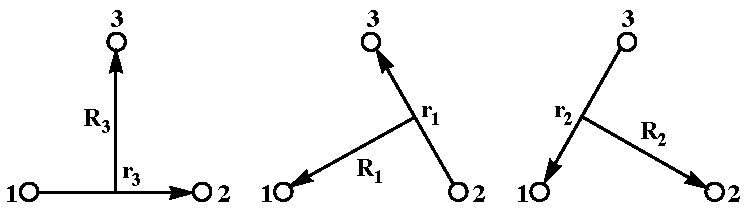
\includegraphics[width=\linewidth]{jacobii.pdf}
	\caption{Illustration of the three different Jacobi coordinate sets.}
	\label{fig:2}
\end{figure}

There are three possible ways to construct the Jacobi coordinates described above, see Figure \ref{fig:2}. Each set transforms into one of the other by exchange of particles. To be able to describe permutations in a system with mass-scaled coordinates it is useful to introduce angles defined by the particle masses \cite{Smith1962}. If an even permutation $(ijk)$ of the set $(123)$ is considered, then the obtuse angle $\beta_{ij}$ has the properties

\begin{subequations}
	\begin{align}
	&\beta_{ij} = -\beta_{ji}, \quad \beta_{ii} = 0,\\
	&\tan\beta_{ij} = -m_k/\mu,\\
	&d_{i}d_{j} \sin\beta_{ij} = 1,\\
	&d_{i}d_{j} m_{k} \cos\beta_{ij} = -\mu,\\
	&\beta_{12}+\beta_{23}+\beta_{31} = 2\pi.
	\end{align}
\end{subequations}
Orthogonal transformations within the coordinate set are then given by 

\begin{equation}
\begin{pmatrix}
\mathbf{r}_j\\
\mathbf{R}_j
\end{pmatrix}
=
\begin{pmatrix}
\cos\beta_{ij} & \sin\beta_{ij}\\
-\sin\beta_{ij} & \cos\beta_{ij}
\end{pmatrix}
\begin{pmatrix}
\mathbf{r}_i\\
\mathbf{R}_i
\end{pmatrix}.
\end{equation}

\section{The Hyperspherical Method}
The next common step in the theoretical framework to describe systems of three particles is to introduce hyperspherical coordinates. The components of the two vectors $\mathbf{r}$ and $\mathbf{R}$ are combined into a single, six-dimensional position vector $\mathbf{q}$. The components of this vector can be regarded as the cartesian components of a point in $\mathbb{R}^{6}$. The motion of a three particle system is thus equivalent to the motion of a single particle, with the reduced mass $\mu$, in six-dimensional Euclidean space. The polar coordinates of this point particle are given by one hyperradial coordinate $\rho$, and five hyperangular coordinates, collectively labelled $\Omega$. Three of these angles $\alpha, \beta, \gamma$ are usually chosen as the Euler angles that specify the  orientation of the body-fixed axis system -- i.e. the triangle formed by the three particles -- relative to a space-fixed coordinate frame. These are the external coordinates of the system. The internal coordinates are the hyperradius -- which describes the overall size of the system -- and the remaining two hyperangles, which describe the shape of the triangle formed by the  three particles. 

Hyperspherical coordinates are useful for describing fragmentation problems. Fragmentation processes of the system into any one of the possible channels are described by the hyperradius becoming very large $(\rho \rightarrow \infty)$, while the hyperangles distinguish between the different fragmentation channels. The hyperradius is invariant under both rotations and particle permutations, and for the three-body problem it is defined by

\begin{equation}
\rho = \Big(\mathbf{r}^{2} + \mathbf{R}^{2}\Big)^{1/2}, \quad 0\leq \rho < \infty.
\end{equation} 

In contrast to the hyperradius there is no unique way to define the hyperangles and the various definitions are not in general invariant under particle permutations. The most common choises of parametrizing the hypersphere fall into two distinct categories: Delves coordinates, and (democratic) Smith-Whitten coordinates. 

\subsubsection{Delves Coordinates}\label{delvescoord}
Delves coordinates are adapted to collinear atom-diatom collisions and are regular polar coordinates. They where originally developed to treat nuclear three-body problems. Each coordinate set is defined by the Jacobi vectors

\begin{align}
r_{k} &= \rho \sin{\alpha_{k}},\\
R_{k} &= \rho \cos{\alpha_{k}},
\end{align}
where the Delves hyperangle $\alpha_{k}$, which correlates to the lengths of these vectors, is defined by

\begin{equation}
\alpha_{k} = \arctan\bigg(\frac{r_{k}}{R_{k}}\bigg), \quad 0\leq \alpha_{k} \leq \frac{\pi}{2}.
\end{equation}
This coordinate set corresponds to the reactant arrangement when particle $k$ scatters off the weakly bound particles $ij$. The other angle in this set is the angle between the two vectors $\mathbf{r}_{k}$ and $\mathbf{R}_{k}$. It is given by

\begin{equation}
\cos{\theta_{k}} = \frac{\mathbf{r}_{k} \cdot \mathbf{R}_{k}}{r_{k} R_{k}}, \quad  0\leq \theta \leq \pi.
\end{equation}
For simplicity, the indicies labelling each coordinate set will be surpressed from hereon. 

The full derivation of the three-body Schr{\"o}dinger equation written in Delves coordinates is given in \cref{delves}, here we simply state the results. After rescaling the total wave function, $\psi = \rho^{5/2}\sin2\alpha\Psi$, the Schr{\"o}dinger equation can be written

\begin{equation}
\bigg(-\frac{1}{2\mu}\frac{\partial^2}{\partial\rho^2} + \frac{\Lambda^2 - 1/4}{2\mu\rho^2} + V(\rho,\alpha,\theta)\bigg) \psi(\rho,\alpha,\theta) = E \psi(\rho,\alpha,\theta),
\end{equation}
in which $E$ is the internal energy and where the squared grand angular momentum operator $\Lambda^2$, which contains all angular variables, is given by

\begin{equation}
\Lambda^2 = -\frac{\partial^2}{\partial\alpha^2} - \frac{1}{\sin^2\alpha\cos^2\alpha\sin\theta} \frac{\partial}{\partial\theta} \bigg( \sin\theta \frac{\partial}{\partial\theta}\bigg).
\end{equation}
The corresponding volume element is proportional to $\rho^5\sin^2\alpha\cos^2\alpha\sin\theta d\rho d\alpha d\theta$. To be square-integrable, the rescaled wavefunction for a bound state must obey the boundary conditions

\begin{align}
\psi(0,\alpha,\theta) &= 0,\\
\psi(\rho,0,\theta)    &= \psi(\rho,\frac{\pi}{2},\theta) = 0,\\
\frac{\partial\psi}{\partial\theta}\bigg\rvert_{\theta = 0} &= \frac{\partial\psi}{\partial\theta}\bigg\rvert_{\theta = \pi} = 0.
\end{align} 

Numerical difficulties arise with these coordinates when permutation symmetries for three identical particles is considered \cite{rimondo_berman_lin}. 

%TODO Utveckla den här biten, skriv om fördelar och nackdelar.   
\subsubsection{Smith-Whitten Coordinates}\label{smith_whitten}
The motion of three particles can be represented in a symmetric way by using so called democratic coordinates. The main advantage with these kind of coordinates is that permutation symmetries for three identical particles can be imposed exactly. To define the two hyperangles $\theta$ and $\phi$ we use the mapping procedure described by Johnson \cite{Johnson1980} to produce a modified set of the coordinates first introduced by Smith and Whitten \cite{Smith_Whitten1968}. The 

\begin{align}
\varphi_1 &= 2\tan^{-1}(m_2/\mu)\\
\varphi_2 &= 2\tan^{-1}(m_1/\mu)
\end{align}
Now we redefine $\phi'_k = \phi_k+7\pi/2$, so that the range is $0 \leq \phi'_k < 4\pi$. Then $\sin\phi_k = \cos\phi'_k$. We finally get ($2\Phi = 4\pi - \phi'$)

\begin{align}
r_3 &= \frac{d_3\rho}{2^{1/2}}\big[1+\sin\theta\cos\phi'\big]^{1/2}\\
r_1 &= \frac{d_1\rho}{2^{1/2}}\big[1 + \sin\theta\cos(\phi'-\varphi_1)\big]^{1/2}\\
r_2 &= \frac{d_1\rho}{2^{1/2}}\big[1 + \sin\theta\cos(\phi' + \varphi_2)\big]^{1/2}.
\end{align}


Now, we make a transformation of the angles (Kuppermann)


and we get the final expression for the Hamiltonian

\begin{align}
H &= -\frac{\hbar^{2}}{2 \mu} \Bigg[ -\frac{15}{4} \frac{1}{\rho^{2}} + \frac{\partial^{2}}{\partial \rho^{2}}+ \frac{4}{\rho^{2}}\Big( \frac{1}{\sin(2\theta)} \frac{\partial}{\partial \theta} \sin(2\theta) \frac{\partial}{\partial \theta} + \frac{1}{\sin^{2}(\theta)} \frac{\partial^{2}}{\partial \phi^{2}} \Big) \Bigg] + V(\rho, \theta, \phi)\\
&= -\frac{\hbar^{2}}{2 \mu \rho^{2} }\frac{\partial^2}{\partial \rho^2} + \frac{\hbar^{2}}{2 \mu \rho^{2} } \Bigg(\Lambda^2 + \frac{15}{4}\Bigg)+ V(\rho, \theta, \phi),
\end{align}
where $\Lambda^2$ is the grand angular momentum operator. 



\section{Adiabatic Hyperspherical Method}\label{sec:AHM}
In the following sections we have chosen to work in the set of democratic hyperangles described in \ref{smith}. With these coordinates, the Schr{\"o}dinger equation for the internal coordinates was derived as  

\begin{equation}\label{schrodinger}
\Bigg(-\frac{1}{2 \mu}\frac{\partial^2}{ \partial \rho^2} + \frac{\Lambda^2 + 15/4}{2 \mu \rho^2} + V(\rho,\theta,\phi) \Bigg)\psi(\rho,\theta,\phi) = E\psi(\rho,\theta,\phi),
\end{equation}
with boundary conditions

\begin{align}
\frac{\partial\Phi_{\nu}(\rho;0,\phi)}{\partial \theta} = \frac{\partial\Phi_{\nu}(\rho;\frac{\pi}{2},\phi)}{\partial \theta},\\
\frac{\partial\Phi_{\nu}(\rho;\theta,0)}{\partial \phi} = \frac{\partial\Phi_{\nu}(\rho;\theta,\frac{2\pi}{3})}{\partial \phi},
\end{align}
reflecting three identical particle symmetry. We assume that the interactions $V$ can be written as a sum of pairwise two-body potentials   

\begin{equation}\label{eq:potential_sum}
V(\rho,\theta,\psi) = v(r_{k}) + v(r_{i}) + v(r_{j}).
\end{equation}
The two-body interaction 

\begin{equation}\label{eq:two_b_potential}
v(r) = d\cosh^{-2}{(r/r_0)}.
\end{equation}

The general feature of the Efimov effect is that it is insensitive to the details of the interatomic interaction. Describe why it is okey to use model potentials, controlling the number of bound two-body systems, controlling the scattering length, tuning trough poles in the scattering matrix.

\begin{align}
r_3 &= 3^{-1/4}\rho [1+\sin \theta \cos \phi]^{1/2} \\
r_1 &= 3^{-1/4}\rho [1+\sin \theta \cos (\phi - 2\pi/3)]^{1/2} \\
r_2 &= 3^{-1/4}\rho [1+\sin \theta \cos (\phi + 2\pi/3)]^{1/2} 
\end{align}
The exact solution to \eqref{schrodinger} can be found by first writing $\psi_{n}(\rho,\theta,\phi)$ as an expansion of radial wavefunctions $F_{\nu n}(\rho)$ and a set of complete, orthonormal channel functions $\Phi_{\nu}(\rho;\theta,\phi)$ that depend parametrically on $\rho$,

\begin{equation}\label{wave}
\psi_{n}(\rho,\theta,\phi) = \sum_{\nu=0}^{\infty} F_{n\nu}(\rho)\Phi_{\nu}(\rho;\theta,\phi).
\end{equation}
The channel functions $\Phi_{\nu}$ are solutions to the hyperangular part of \eqref{schrodinger}

\begin{equation}\label{adiabatic}
\bigg(\frac{\Lambda^2+15/4}{2 \mu_{3} \rho^2} + V(\rho,\theta,\phi)\bigg) \Phi_{\nu}{(\rho;\theta,\phi)}= U_{\nu}{(\rho)} \Phi_{\nu}(\rho;\theta,\phi),
\end{equation}
and $U_{\nu}(\rho)$ are the resulting effective potental curves obtained by solving this eigenvalue equation at a number of different hyperradii. Substituting \eqref{wave} into \eqref{schrodinger} and projecting out $\Phi_{\nu'}$ by multiplying the conjugate transpose $\Phi_{\nu}^{\dagger}$ to the left and integrating over the hyperanglular coordinates results in an infinite set of coupled differential equation in $\rho$, which reads

\begin{align}\label{fullhamiltonian}
\bigg(-\frac{1}{2 \mu}\frac{\partial^2}{ \partial \rho^2} + U_{\mu}(\rho) - \frac{1}{2\mu}Q_{\mu\mu}(\rho) \bigg)F_{n\mu}(\rho)&\nonumber\\ -\frac{1}{2\mu}\bigg(\sum_{\nu\neq\mu}2P_{\mu\nu}(\rho)\frac{\partial}{\partial\rho} + Q_{\mu\nu}(\rho) \bigg)F_{n\nu}(\rho)& = E_nF_{n\mu}(\rho),
\end{align}
where the nonadiabatic coupling terms $P_{\mu\nu}$ and $Q_{\mu\nu}$ involve partial first and second derivative of the channel functions with respect to $\rho$. They are generated by the $\rho$ dependence of the channel functions and are defined as 

\begin{equation}\label{couplingP}
P_{\mu\nu}(\rho) = \llangle[\Big]  \Phi_{\mu} \Big\lvert \frac{\partial}{\partial\rho} \Big\rvert  \Phi_{\nu} \rrangle[\Big],
\end{equation}
and

\begin{equation}\label{couplingQ}
Q_{\mu\nu}(\rho) = \llangle[\Big]  \Phi_{\mu} \Big\lvert \frac{\partial^2}{\partial\rho^2} \Big\rvert  \Phi_{\nu} \rrangle[\Big],
\end{equation}
where the double brackets denote integration over the two angular coordinates. Integration by parts, the completeness requirement of the channelfunctions together with the antisymmetric properties of the coupling matrix $P_{\mu \nu}$,  i.e. $P_{\mu \nu}= - P_{\nu \mu}$, are used to derive the following relation 

\begin{equation}
Q_{\mu \nu} = \frac{dP_{\mu \nu}}{d\rho} + P^2_{\mu \nu},
\end{equation}
where the square of the coupling matrix $P_{\mu \nu}$ relates to $Q_{\mu \nu}$ through 

\begin{align}
P^2_{\mu \nu} &= \sum_{\sigma}P_{\mu \sigma}P_{\sigma \nu} = \sum_{\sigma}\llangle[\Big] \Phi_{\mu} \Big\lvert \frac{\partial \Phi_{\sigma}}{\partial\rho}  \rrangle[\Big]\llangle[\Big] \Phi_{\sigma} \Big\lvert \frac{\partial \Phi_{\nu}}{\partial\rho}  \rrangle[\Big]\nonumber\\
&=\sum_{\sigma}-\llangle[\Big]\frac{\partial \Phi_{\mu}}{\partial\rho} \Big\lvert  \Phi_{\sigma} \rrangle[\Big]\llangle[\Big] \Phi_{\sigma} \Big\lvert \frac{\partial \Phi_{\nu}}{\partial\rho}  \rrangle[\Big]=- \llangle[\Big] \frac{\partial \Phi_{\mu}}{\partial \rho}  \Big\lvert \frac{\partial \Phi_{\nu}}{\partial\rho}  \rrangle[\Big].
\end{align}
The antisymmetry of $P_{\mu\nu}$ together with $P_{\mu\nu}^2 = P_{\nu\mu}^2$ leads to $P_{\nu\nu} = 0$ and $Q_{\nu \nu} = P_{\nu\nu}^2$. 

In the adiabatic hyperspherical approximation the diagonal elements are neglected and the effective potentials are defined as

\begin{equation}
W_{\nu}(\rho) = U_{\nu}(\rho)-\frac{1}{2\mu}Q_{\nu \nu}(\rho) = U_{\nu}(\rho)-\frac{1}{2\mu}P_{\nu \nu}^2(\rho).
\end{equation} 
The hyperspherical Born-Oppenheimer approximation, the effective potentials are simply $U_{\nu}(\rho)$, thus neglecting the diagonal terms. 

\begin{equation}
W_{\nu}(\rho) = -\frac{s_0^2+1/4}{2\mu \rho^2}.
\end{equation} 


\section{Generalized Hellmann-Feynman theorem}
The following subsection concerns the mathematical description of the non-adiabatic coupling matrices that was defined in subsection \ref{sec:AHM}. To obtain an expression for the coupling term $P_{\mu \nu}$ given in \eqref{couplingP}, a generalized Hellmann-Feynman (HF) approach can be used. Consider $\nu$ adiabatic eigenstates $\Phi_{\nu}$, which are obtained by
\begin{equation}\label{HA}
H_{ad}\Phi_{\nu} = U_{\nu}\Phi_{\nu},
\end{equation}
where the adiabatic Hamiltonian $H_{ad}$ is just the hyperangular part of the Schr{\"o}dinger equation given in \eqref{adiabatic}, and the eigenvalues $U_{\nu}(\rho)$ are the effective adiabatic three-body potential curves. Using the identities 

\begin{align}
\llangle[\big]  \Phi_{\mu} \big\rvert  \Phi_{\nu}  \rrangle[\big] &\equiv \delta_{\mu \nu}\\
\intertext{and}
\frac{\partial}{\partial \rho}\llangle[\big]  \Phi_{\nu}  \big\rvert  \Phi_{\nu} \rrangle[\big] &\equiv 0,
\end{align}
we start by deriving the diagonal part of the HF theorem. Projecting $\Phi_{\nu}$ out from equation \eqref{HA}, and differentiating with respect to the hyperradius gives

\begin{align}
\frac{\partial U_{\nu}}{\partial \rho}&=\frac{\partial}{\partial \rho}\llangle[\big]  \Phi_{\nu} \big\lvert H_{ad} \big\rvert  \Phi_{\nu} \rrangle[\big]\nonumber\\
&=\llangle[\Big]  \Phi_{\nu}  \Big\lvert \frac{\partial H_{ad}}{\partial \rho} \Big\rvert  \Phi_{\nu} \rrangle[\Big] +  \llangle[\Big]  \Phi_{\nu} \Big\lvert H_{ad}\Big\rvert  \frac{\partial \Phi_{\nu}}{\partial \rho}  \rrangle[\Big] +\llangle[\Big] \frac{\partial \Phi_{\nu}}{\partial \rho}    \Big\lvert H_{ad}\Big\rvert  \Phi_{\nu}  \rrangle[\Big] \nonumber \\
&=\llangle[\Big]  \Phi_{\nu} \Big\lvert \frac{\partial H_{ad}}{\partial \rho} \Big\rvert  \Phi_{\nu} \rrangle[\Big] + U_{\nu}\llangle[\Big]  \Phi_{\nu} \Big\rvert \frac{\partial \Phi_{\nu}}{\partial \rho}  \rrangle[\Big]+U_{\nu}\llangle[\Big] \frac{\partial \Phi_{\nu}}{\partial \rho}\Big\rvert  \Phi_{\nu} \rrangle[\Big] \nonumber \\
&=\llangle[\Big]  \Phi_{\nu} \Big\lvert \frac{\partial H_{ad}}{\partial \rho} \Big\rvert  \Phi_{\nu} \rrangle[\Big] + U_{\nu} \frac{\partial}{\partial \rho}\llangle[\Big]  \Phi_{\nu} \Big\rvert \Phi_{\nu} \rrangle[\Big] \nonumber \\
&=\llangle[\Big]  \Phi_{\nu}\Big\lvert \frac{\partial H_{ad}}{\partial \rho} \Big\rvert  \Phi_{\nu} \rrangle[\Big].
\end{align}
The generalized HF theorem also includes the nondiagonal terms. Multiplying with $\Phi_{\mu}^{\dagger}$ to the left of \eqref{HA} and integrating over the two hyperangles, followed by differentiation with respect to the hyperradius gives

\begin{align}
&\frac{\partial U_{\nu}}{\partial \rho}\llangle[\Big]  \Phi_{\mu} \Big\lvert \Phi_{\nu} \rrangle[\Big] + U_{\nu}\llangle[\Big]  \Phi_{\mu} \Big\lvert \frac{\partial \Phi_{\nu}}{\partial \rho} \rrangle[\Big]+U_{\nu}\llangle[\Big] \frac{\partial \Phi_{\mu}}{\partial \rho} \Big\lvert \Phi_{\nu} \rrangle[\Big] \nonumber \\
&= \llangle[\Big]  \Phi_{\mu}\Big\lvert \frac{\partial H_{ad}}{\partial \rho} \Big\rvert  \Phi_{\nu} \rrangle[\Big] + U_{\mu}\llangle[\Big]  \Phi_{\mu} \Big\rvert  \frac{\partial \Phi_{\nu}}{\partial \rho}  \rrangle[\Big]+U_{\nu}\llangle[\Big] \frac{\partial \Phi_{\mu}}{\partial \rho}\Big\rvert  \Phi_{\nu} \rrangle[\Big]. 
\end{align}
The first term on the left side of this equation i zero by the orthogonality of the channel functions. By removing the last term on both sides we obtain the final expression

\begin{equation}\label{derivaham}
\llangle[\bigg]  \Phi_{\mu}\bigg\lvert \frac{\partial H_{ad}}{\partial \rho} \bigg\rvert \Phi_{\nu} \rrangle[\bigg]= \big(U_{\nu}-U_{\mu}\big) \llangle[\bigg]  \Phi_{\mu} \bigg\lvert \frac{\partial}{\partial \rho} \bigg\rvert \Phi_{\nu} \rrangle[\bigg],
\end{equation}
and we can express the nonadiabatic coupling terms $P_{\mu \nu}$ as

\begin{equation}
P_{\mu \nu} = \frac{1}{\big(U_{\nu}-U_{\mu}\big)}\llangle[\bigg]  \Phi_{\mu} \bigg\lvert \frac{\partial H_{ad}}{\partial \rho} \bigg\rvert \Phi_{\nu}\rrangle[\bigg].
\end{equation}
Assume that the channel functions can be expressed as a series of basis functions

\begin{equation}
\Phi_{\nu} = \sum_{j}C_{\nu}^j \varphi_j,
\end{equation} 
Where $C_{\nu}^{j}$ are the expansion coeffients given in TODO(make reference). Anticipating that the Hamiltonian operator will take the matricial form of elements $H_{ij}$. From the results of the diagonal case discussed in, we obtain the following matrical expression \cite{Sanz-Sanz}

\begin{equation}
\frac{\partial U_{\nu}}{\partial \rho} = \sum_{ij}(C_{\nu}^i)^{\dagger}C_{\nu}^j \frac{\partial H_{ij}}{\partial \rho}.
\end{equation}
In the non-diagonal case the result in matrical form reads 

\begin{equation}
\llangle[\bigg]  \Phi_{\mu} \bigg\lvert \frac{\partial}{\partial \rho} \bigg\rvert \Phi_{\nu} \rrangle[\bigg] = P_{\mu \nu} = \sum_{ij}(C_{\mu}^i)^{\dagger}C_{\nu}^j \frac{\partial H_{ij}}{\partial \rho}.
\end{equation}
